% \documentclass{WHUBachelor}% 选项 forprint: 交付打印时添加, 避免彩色链接字迹打印偏淡. 即使用下一行:
 \documentclass[forprint]{WHUBachelor}
  \lstset{ 
    basicstyle=\small,% 
    escapeinside=``,% 
    keywordstyle=\color{red} \bfseries,% \underbar,% 
    identifierstyle={},% 
    commentstyle=\color{blue},% 
    stringstyle=\ttfamily,% 
    %labelstyle=\tiny,% 
    breaklines=true,
    extendedchars=false,% 
    linewidth=\textwidth,% 
    numbers=left,% 
    numberstyle=\tiny \color{blue},% 
    frame=trbl% 
    }


\begin{document}
%%%%%%% 下面的内容, 据实填空.

\title{实验项目一:接管裸机的控制权之自定义引导程序的实现}
\Cschoolname{数据科学与计算机学院}          % 学院名
\Cmajor{计算机科学与技术}                  % 专业中文名
\StudentNumber{16337237} % 填写自己的学号
\author{王永锋}                            % 作者名字
\Csupervisor{凌应标}        %指导教师中文名、职称
\date{二〇一八年三月十日}                    % 日期, 要注意和英文日期一致!!

%----------------------------------------------------------------------------
\pdfbookmark[0]{封面}{title}         % 封面页加到 pdf 书签
\maketitle
\frontmatter
\pagenumbering{Roman}              % 正文之前的页码用大写罗马字母编号.
%-----------------------------------------------------------------------------
% \include{includefile/frontmatter}    % 加入摘要, 申明.
%==========================把目录加入到书签==============================%%%%%%
\pdfbookmark[0]{目录}{toc}
\tableofcontents
\mainmatter %% 以下是正文
%%%%%%%%%%%%%%%%%%%%%%%%%%%--------main matter-------%%%%%%%%%%%%%%%%%%%%%%%%%%%%%%%%%%%%
\chapter{实验目的及要求}

\section{实验目的}

\begin{enumerate}
  \item 学会使用虚拟机启动DOS引导盘,并使用DOS引导盘运行16位的汇编程序。
  \item 学会使用winhex修改磁盘镜像文件。
  \item 学会使用nasm编译x86汇编程序。
  \item 能够自己独立编写引导程序,并能引导虚拟机正常启动。
\end{enumerate}

\section{实验要求}

本次实验,要求需要完成以下目标:\\

\begin{itemize}
  \item \textbf{搭建和应用实验环境} \\
  虚拟机安装,生成一个基本配置的虚拟机PC和多个1.44MB容量的虚拟软盘,将其中一个虚拟软盘用DOS格式化为DOS引导盘,用WinHex工具将其中一个虚拟软盘的首扇区填满你的个人信息。
  \item \textbf{接管裸机的控制权} \\
  设计IBM\_PC的一个引导扇区程序,程序功能是:用字符‘A’从屏幕左边某行位置45度角下斜射出,保持一个可观察的适当速度直线运动,碰到屏幕的边后产生反射,改变方向运动,如此类推,不断运动;在此基础上,增加你的个性扩展,如同时控制两个运动的轨迹,或炫酷动态变色,个性画面,如此等等,自由不限。还要在屏幕某个区域特别的方式显示你的学号姓名等个人信息。将这个程序的机器码放进放进第三张虚拟软盘的首扇区,并用此软盘引导你的PC,直到成功。
\end{itemize}

\chapter{实验1方案:搭建和应用实验环境}

% \section{相关基础原理}

\section{实验工具和环境}

本次实验平台(部分参考\cite{于渊2009orange}搭建在win10系统上,通过编写shell脚本,连接nasm编译工具,dd二进制文件覆写工具,与bochs虚拟机加载配置文件与镜像(具体工具链详见下\autoref{tab:tools},实现了\textbf{编写代码后一键启动虚拟机查看结果}。同时,使用bochs虚拟机中提供的bochsdbg.exe工具,还能够对产生的镜像文件进行\textbf{单步调试},不仅大大提高了编写汇编文件后查看实现效果的速度,在命令行中通过发送指令对虚拟机的运行进行单步调试,查看各寄存器和内存,能够迅速定位操作系统中存在的问题并且解决它,从而提高我们的开发效率。考虑到bochs虚拟机由于是软件模拟硬件,速度不仅不稳定而且比较慢,因此后来我采用qemu虚拟机进行查看引导程序的结果。

\begin{table}[htp]
  \caption{本实验所使用的工具链}
  \centering
  \begin{tabular}{cc}
    \toprule
    软件名称 & 用途  \\
    \midrule
    bash & 一个命令行终端,可提供linux的一些命令与执行shell脚本 \\
    nasm & 将x86汇编文件编译成.bin二进制文件 \\
    dd & 将二进制文件的内容写进软盘镜像中  \\
    winhex & 以二进制形式查看及修改软盘镜像文件 \\
    bochs & 虚拟机,用于加载装有自定义引导程序的软盘  \\
    bochsdbg & 调试工具,用于给装有自定义引导程序的软盘文件进行调试 \\
    qemu & 虚拟机,用于加载装有自定义程序的软盘 \\
    \bottomrule
  \end{tabular}
  \label{tab:tools}
\end{table}





\section{制作DOS引导盘并启动}

\subsection{操作步骤}

\begin{description}
  \item [步骤 1] 从bochs官网上,找到了FreeDOS的镜像文件。
  \item [步骤 2] 修改bochs虚拟机的配置文件,使其指向刚下载的镜像文件。
  \item [步骤 3] 使用bochs打开FreeDOS,并进行简单的使用与实验。
\end{description}

\subsection{操作结果}

操作结果,详见\autoref{fig:freeDOS}。
\begin{figure}[htp]
  \centering
  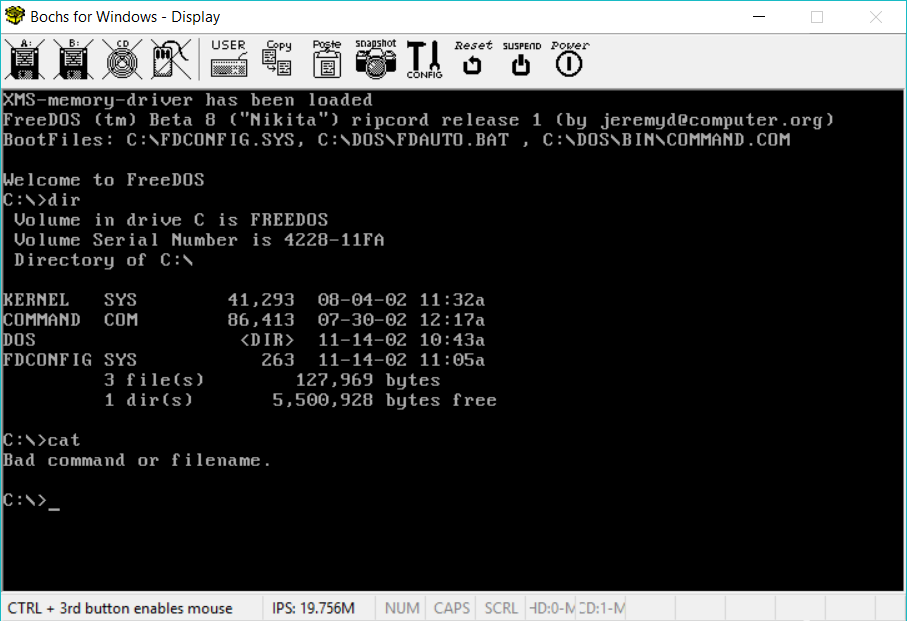
\includegraphics[width=13cm]{"./figure/use_freeDOS.png"}
  \caption{使用bochs加载freeDOS镜像的截图}
  \label{fig:freeDOS}
\end{figure}

\section{使用个人信息填满引导扇区}

\subsection{操作步骤}

\begin{description}
  \item [步骤 1 : 编写代码,生成填满个人信息的二进制文件。] 

  考虑到个人信息需要填满软盘第一个扇区的前512个字节,手工复制粘贴费时费力,在这里我采用times语句,将我的个人信息复制100次之后生成二进制文件。代码如下所示。
  \label{code:generate_infomation}
  \begin{lstlisting}
times 100 dw '16337237 wang yong feng'
  \end{lstlisting}

  \item [步骤 2 : 使用dd工具,将生成的二进制文件写到软盘镜像中。] 
  
  在命令行下,可以使用这样的命令进行二进制文件的覆写。

  \begin{lstlisting}
dd if=a.bin of=a.img bs=512 count=1 conv=notrunc
  \end{lstlisting}

  \item [步骤 3] 使用WinHex工具,查看修改后的二进制文件是否已经被成功覆写,并确认覆写结果是否正确。
\end{description}

\subsection{操作结果}

个人信息“16337237 wang yong feng"成功填充到软盘镜像文件中,如\autoref{fig:information}所示

\begin{figure}[htp]
  \centering
  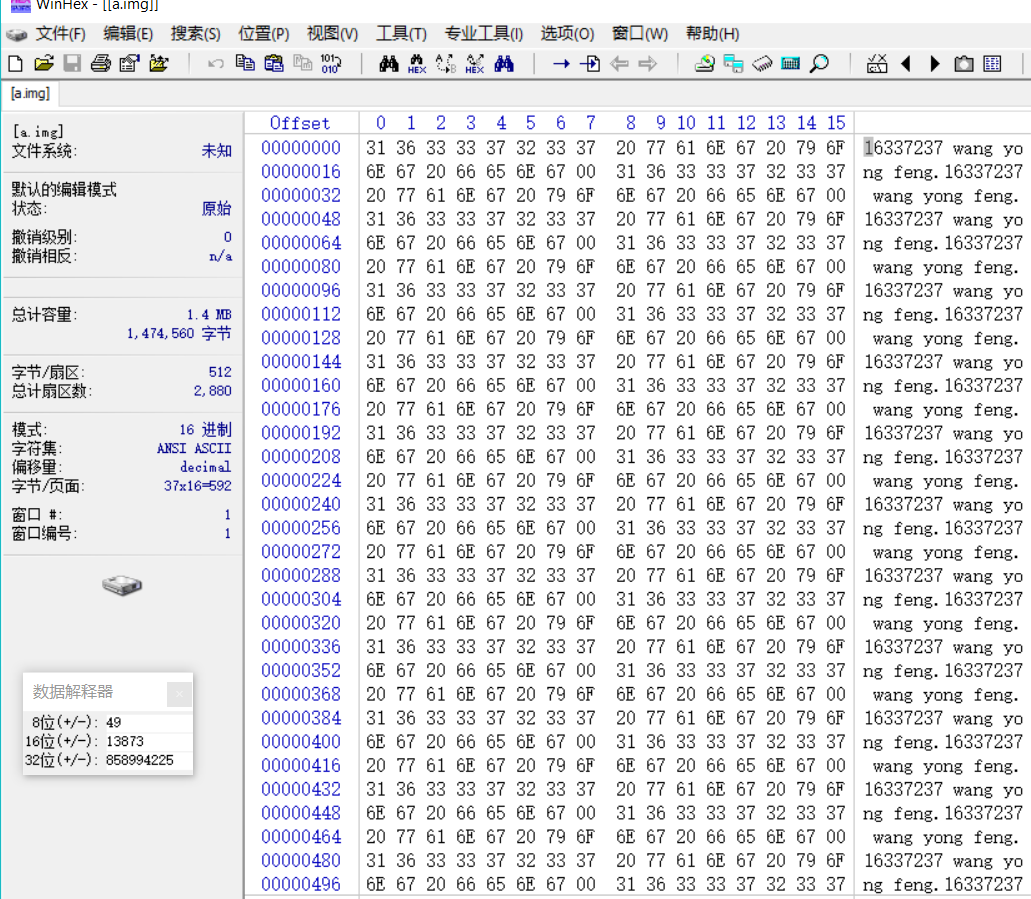
\includegraphics[width=14cm]{"./figure/information.png"}
  \caption{使用winhex查看填充个人信息后的软盘镜像第一扇区}
  \label{fig:information}
\end{figure}


\chapter{实验2方案:自定义引导程序的实现}

\section{相关基础原理}

本次实验能够成功进行,离不开这些基础原理的支撑。

\subsection{电脑开机流程与主引导扇区}

计算机开机后,访问硬盘时所必须要读取的首个扇区称为主引导扇区\cite{wiki:mainbootrecord}。在BIOS的调控下,计算机会寻找到在第511和512个字节处为55aa的磁盘,并认定该盘为引导盘,从而将该盘的第一个扇区加载进内存的0000:7c00处,并将CPU的控制权交给位于内存地址0000:7c00处的指令,这就是我们这一次实验要实现的位于引导盘主引导扇区中的引导程序。

因此,加载进内存的位置由于历史遗留问题,固定在了0000:7c00处,因此,我们的汇编代码中,必须加上如下的一条:
\begin{lstlisting}
org 7c00h
\end{lstlisting}
来确保汇编代码中的绝对地址在运行时仍然保持正确。


\subsection{显存与显示模式}

显卡都有自己的显示存储器,我们要控制显示输出,只需要往显存写入响应的数据即可。对于显存的读写交互,系统将显示存储器映射到了内存中的0000:B800:0000:FFFF中,因此,我们只需要对内存中的这一段地址进行操作,即可控制显示的输出\cite{2013x86汇编语言从实模式到保护模式} 。如\autoref{fig:display_store}所示。

\begin{figure}[htp]
  \centering
  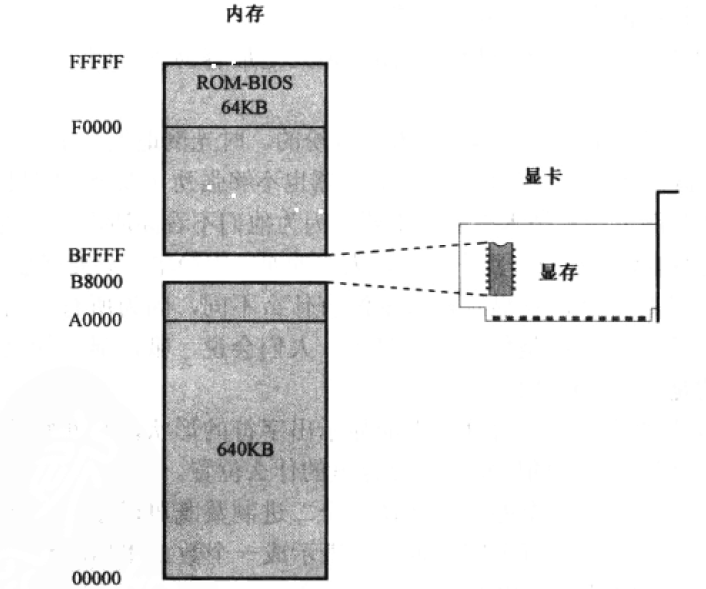
\includegraphics[width=7cm]{"./figure/display_store.png"}
  \caption{文本模式下x显存到内存的映射}
  \label{fig:display_store}
\end{figure}

对显存进行操作的时候,我们还需要知道,在文本模式下,能够显示的字符有80*25个,并且,每一个字符的显示,都需要操作两个字节。第一个字节为该字符的ascii码,而第二个字符为该字符的显示格式。显示格式相关资料可在网上或书中找到,此处不多加赘述。

\begin{figure}[htp]
  \centering
  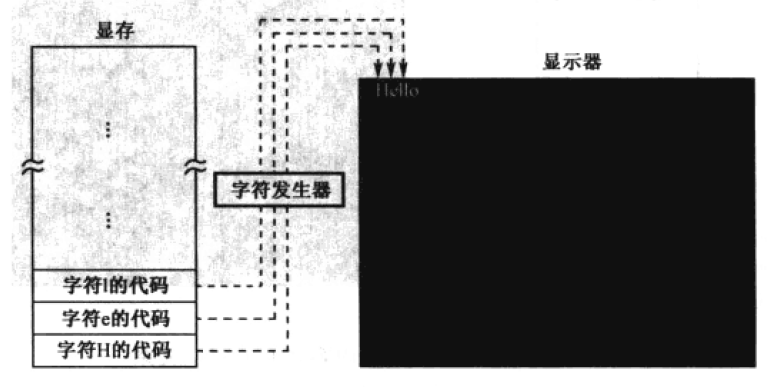
\includegraphics[width=7cm]{"./figure/display_text_mode.png"}
  \caption{字符在屏幕上的显示原理}
  \label{fig:display_text_mode}
\end{figure}


\subsection{几个在汇编程序中用到的中断}\label{sub:interrupt}

在本实验中,有两个软中断的作用显得尤为关键:

\begin{itemize}
  \item \textbf{int 16h} :用于控制键盘操作。
  \item \textbf{int 13h} :用于将磁盘内容写进内存。
\end{itemize}

以下是相关中断的详细说明

\begin{enumerate}

  \item \textbf{int 16h 0号中断} 可从键盘缓冲区中读取一个按键信号,其中扫描法放在ah,按键对应ascII码放在al。在这一次实验中,主要就是用int 16h 0号中断,从al中读取按键对应的ascII码,从而实现根据按键选择功能的效果。

  \item \textbf{int 16h 1号中断} 不断的检测键盘缓冲区。一旦检测到键盘缓冲区有输入,会将标志寄存器中的zf置为1。在本次实验中,就是通过一个循环不停地检测键盘缓冲区,来实现对键盘操作的实时回应。

  \item \textbf{int 13h 2号中断} 该中断可以将磁盘的某一个或几个扇区加载进内存的一个特定的位置中。该终端所需参数比较多,可见\autoref{tab:int13h}。

\begin{table}[htp]
  \caption{INT 13h 2号中断所需参数列表}
  \centering
  \begin{tabular}{cc}
    \toprule
    参数对应寄存器 & 相应应该放入的参数类型 \\
    \midrule
    AH & 中断号 02h \\     
    AL & 一次中断读取的扇区数目 \\
    CH &	起始磁道 \\
    CL &	起始扇区 \\
    DH &	磁头号 \\
    DL &	驱动器号 \\
    ES:BX & 写进内存的地址 \\	    
    \bottomrule
  \end{tabular}
  \label{tab:int13h}
\end{table}


\end{enumerate}


\section{实验工具和环境}
此处不赘述,可见前文\autoref{tab:tools}。

\section{程序功能说明}

本程序(完整程序代码见附件)在主引导扇区及第二第三扇区中编写的程序实现了以下功能(主界面可见\autoref{fig:main_screen})。

\begin{enumerate}
  \item 有一个跳动的颜色会变的笑脸会在屏幕上跳来跳去,一旦遇到边缘则反弹。
  \item 右下角有我自己的学号和姓名的拼音。
  \item 键盘按下C,可实现清屏(不清学号和姓名)
  \item 键盘按下D,可通过字符画的形式在80*25有限的空间内展示我名字的汉字形式。可见\autoref{fig:main_screen2}
\end{enumerate}



\chapter{实验结果}
本程序经nasm编译后在bochs虚拟机下运行的效果可见\autoref{fig:main_screen}与\autoref{fig:main_screen2}

通过完成本实验,我们完成了以下工作,验证了以下结论:

\begin{enumerate}
  \item 搭建了一套完整的,支持32位汇编代码编写的,且高效率的操作系统开发环境,并在实验的过程中进一步熟悉了该开发环境与调试工具的使用。
  \item 验证了书本上所说的电脑开机时所做的一部分工作,如选择引导盘是通过选择第一个扇区末尾为0x55aa来判断的,如会将主引导扇区加载到内存地址为0000:7c00的位置中,通过自己的探索,也找到了通过主引导扇区中的引导程序,加载在磁盘其他位置的系统内核的方法。
\end{enumerate}

\begin{figure}[htp]
  \centering
  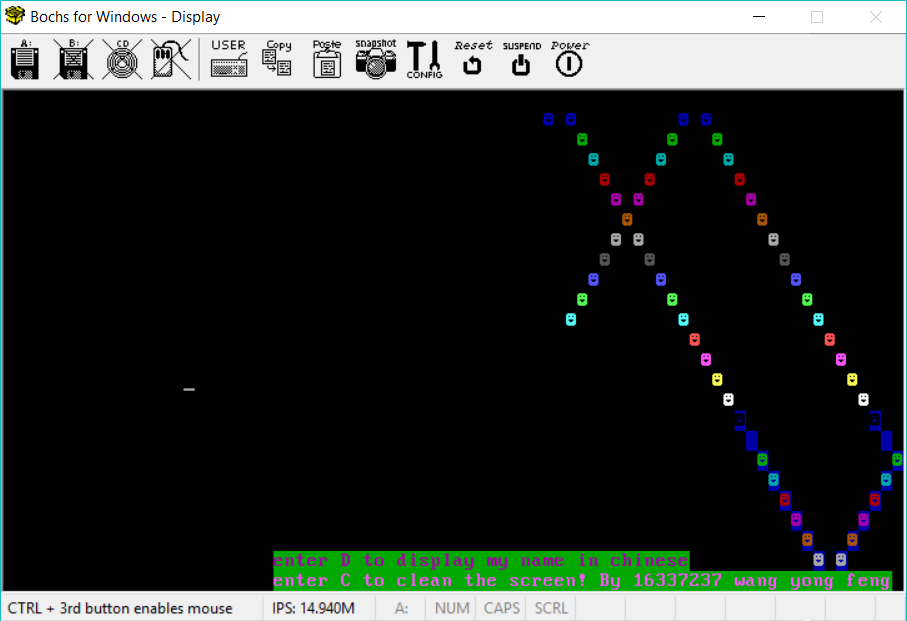
\includegraphics[width=16cm]{"./figure/main_screen.png"}
  \caption{自定义引导程序的主界面}
  \label{fig:main_screen}
\end{figure}

\begin{figure}[htp]
  \centering
  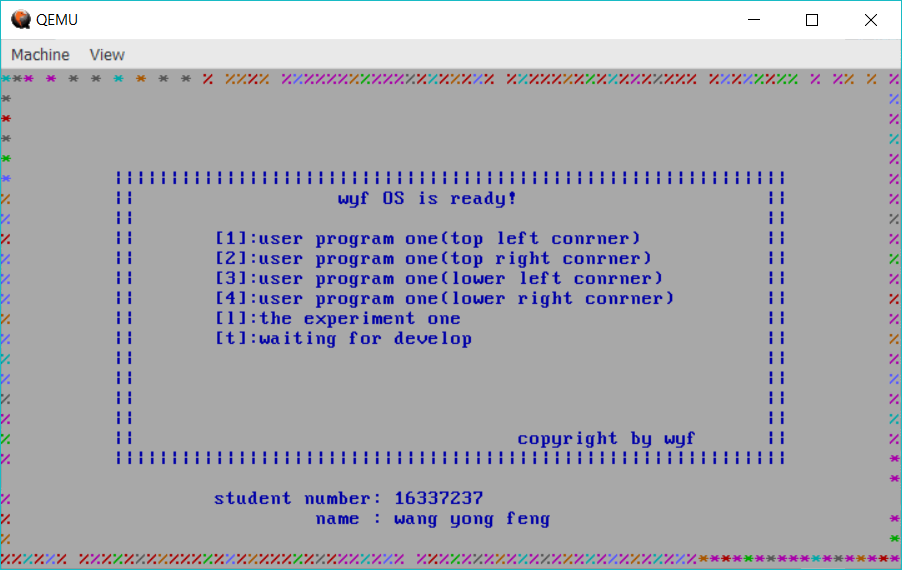
\includegraphics[width=16cm]{"./figure/main_screen2.png"}
  \caption{自定义引导程序按下D后的界面}
  \label{fig:main_screen2}
\end{figure}


\chapter{实验总结}

这是第一次操作系统实验,也是我第一次使用汇编语言直接对硬件进行操作(虽然是虚拟的硬件)。
其实,我们现在对操作系统的学习的门槛已经降低了很多,这首先要归功于在主板上已经内置写好的BIOS引导程序,有了这个引导程序,才能够进一步将CPU的控制权交给到我们能够直接编程的引导盘的主引导扇区,我们才能够做到“接管裸机的控制权”。

由于有过一些x86汇编语言的基础,在实验刚开始进行的时候其实问题还不太大,上学期的计算机组成原理课程中,我曾经使用X86汇编语言与masn汇编器,实现了一个很简单的小游戏,在这个过程中,对中断的理解也加深了很多。也正是有过之前的经历,这一次才能够大胆地将中断用在引导程序中。

但是说这个实验很简单,那暂时还是不可能的。由于平时用汇编语言还比较少,加上这一次使用的工具是nasm,一个更为先进也更为优良的汇编器,与我原本用的masm在语法上有一点点区别,我还是花了一些时间取看nasm的官方文档,来去尽快的适应新的汇编器。值得庆幸的是,nasm的官方文档里面就有一节就是写给用过masm的人,为了他们更快的适应nasm。由此可见,在不熟悉的工具面前,官方的文档比起网上的各种博客而言,往往有效而又全面得多。

但是这个实验的成功,还得归功于我相对比较好的资料检索能力与独立解决问题的能力。512个字节的限制,应该说是阻挡了大多数有意思的想法,一开始的我甚至想着就简简单单的完成实验基本要求就好。还好后来,自己的好奇推动了自己进一步往前探索:“肯定有办法加载其他扇区的内容啊,不然操作系统的内核怎么加载进来的?”,在网上找了很多理论上的资料都没有讲到这方面的解决方法,后来终于发现,是自己搜索问题的关键词不太恰当。换了一下关键词,很快就找到了自己的问题的解决方法。

还有一点想说的是,在开发操作系统的过程上,开发效率是非常重要的一点。影响开发效率有两个重要的因素,一个是修改代码后显示效果的时间,另一个是遇到问题后定位问题的途径多少。

为了能够达到修改代码后能够一键打开虚拟机查看结果,我在自己原有的一点shell编程经验的基础上,完成了一个比较简单的脚本用于一键打开虚拟机查看结果。有时候我看到有同学先输入命令行编译,然后打开winhex复制粘贴二进制代码,然后另存为镜像文件,然后打开vmware虚拟机跑,这一系列的过程需要比较多繁琐的键盘和鼠标的操作。虽然说这些操作也并不是那么繁杂,但是当调试达到一定次数,这种操作的烦躁确乎会影响自己学习的积极性。因此,想了一下,这一套方案还是有必要向同学们推广一下。

遇到问题,是一件很常见的事情,但是我们有多少种方式可以去定位问题的所在呢?光靠编译输出查看结果的确是一个途径,但是这个途径能够提供给我们的信息实在是太少了,我们只能够看到显示在显示屏的显存的情况,但是对CPU的各种内部的参数,却完全没有任何获知的渠道。此时,一个类似于gdb的调试工具就显得尤为必要。因此,我选择bochs虚拟机的另外一个理由也是因为它为我们提供了一个堪比gdb般好用的bochsdbg.exe。这一次实验的完成,中间很多问题的定位,都是多亏了这个工具给我的信息(包括查看各种内部寄存器,内存内容)我才能够准确地定位问题。同时也用这一套工具,帮了个别同学检查他们代码中的问题。

这一次实验,还是给了我不少收获的,在做实验的中间,也查找了不少资料,大体想来,对操作系统原理的理解又深了一些。下一次继续加油吧。

\chapter{实验难点及亮点}

\section{突破主引导扇区512字节的限制}

在设计功能并且尝试实现的过程中,我发现一旦我写的代码多了一点,就很容易导致代码长度超出512个字节,进而导致我的代码不能够被正确的执行。这是一个很严重的问题,这导致我不能够自由的添加我想要实现的功能。经过上网搜索,在网友的CSDN博客\cite{noauthor_boot_nodate}中,找到了相关的解决方法,我们可以使用x86中自带的int 13h中断\cite{wiki:int13}中的2号中断,将第二个扇区及之后的数据加载进原来代码段之后的那一段内存中。相关参数说明也可在\autoref{sub:interrupt}中找到。以下为我在引导扇区中编写的加载第2~8个扇区的代码。

\begin{lstlisting}[language={[x86masm]Assembler}] 
load_os:
  mov ah,02h                            ;读磁盘扇区
  mov al,07h                            ;读取7个扇区
  mov ch,00h                            ;起始磁道
  mov cl,02h                            ;起始扇区
  mov dh,00h                            ;磁头号
  mov dl,00h                            ;驱动器号
  mov bx,os                             ;os为标签,地址为第二扇区的第一个字节
  int 13h
  ret
\end{lstlisting}

在调用该过程之后,在第一个扇区之后的代码就可以加载进内存,从而顺利执行,突破了512字节的限制,而这与引导程序加载系统内核的原理相同。

\section{读取键盘的操作}

我设计的功能中,涉及到与键盘之间的交互,比如通过按C来进行清屏。读取键盘的功能,是通过~int16h~中断实现的。但是这里有个问题,我希望我写的引导程序能够时时刻刻都能够响应我对键盘的操作,但是引导程序又不能够停止运行,也就是说,\textbf{不能够让读取键盘的操作阻塞主界面中笑脸的移动。} 

为了解决这个问题,我在编写代码的时候,设计了一个循环用于检测是否有操作键盘,在检测的时候还要去执行响应的笑脸移动过程(loop1),以及显示学号姓名过程(display\_infomation)。实现的代码如下:

\begin{lstlisting}[language={[x86masm]Assembler}] 
check_keyboard:
  call loop1
  call display_infomation
  call display_message
  mov ah, 01
  int 16h
  ; 如果没有按, zf为0P
  ; 如果有按,往下执行
  jz check_keyboard

  ; 当检测到按键,判断按键是否需要响应,以及决定响应的功能
  ; 从键盘读入字符,扫描码读进ah,ascII码读进al
  mov ah, 00h
  int 16h
  ; 判断字符
  cmp al, 'c'
  mov word [status], 0720h
  jnz check_keyboard_d 
  call clean_screen
  jmp check_keyboard
  check_keyboard_d:
  cmp al, 'd'
  jnz check_keyboard_h
  call clean_screen
  call display_chinese_name
  jmp check_keyboard
  check_keyboard_h:
  jmp check_keyboard
\end{lstlisting}
 
\section{源程序中的一处不完善的地方}

老师给的源代码实现了一个简单的asiII字符的移动与遇墙反弹,但是在程序的开发调试过程中,我发现了这个程序有一个比较严重的漏洞。当该字符移动到墙角的时候,字符所在的位置可能会越界,这会导致字符的x,y坐标与字符实际处在的位置不相符合,原先遇墙反弹的效果也会消失,变成了隔一段时间字符出现一次。






%%%============================================================================================================%%%

%%%=== 参考文献 ========%%%



% \cleardoublepage\phantomsection
% \addcontentsline{toc}{chapter}{参考文献}

\bibliography{opsystem}
% \bibliographystyle{unsrt}

% \begin{thebibliography}{00}

%   \bibitem{r1} 作者. 文章题目 [J].  期刊名, 出版年份,卷号(期数): 起止页码.

%   \bibitem{r2} 作者. 书名 [M]. 版次. 出版地:出版单位,出版年份:起止页码.

%   \bibitem{r3} 邓建松等, 《\LaTeXe~科技排版指南》, 科学出版社.

%   \bibitem{r4} 吴凌云, 《CTeX~FAQ (常见问题集)》, \textit{Version~0.4}, June 21, 2004.

%   \bibitem{r5} Herbert Vo\ss, Mathmode, \url{http://www.tex.ac.uk/ctan/info/math/voss/mathmode/Mathmode.pdf}.


% \end{thebibliography}

% \include{includefile/backmatter} %%%致谢

%%%-------------- 附录. 不需要可以删除.-----------
\appendix

\chapter{运行汇编文件的脚本}

这是我为了方便,在win10平台下的bash终端编写的shell脚本。
\begin{lstlisting}
name=$1
nasm -f bin -l $1.list $1.asm -o $1.bin
# add the feature : if the image not exist, create the image
if [ ! -f "a.img" ]
then
    echo "a.img not exist!"
    echo "use bximage to create a image";
    exit
else
    echo "a.img exists !"
fi
dd if=$1.bin of=a.img bs=512 count=1 conv=notrunc
if [ ! -f "bochsrc.bxrc" ]
then
    echo "bochsrc.bxrc not exist!"
    echo "copy a bochsrc.bxrc to this path quickly";
    exit
else
    echo "bochsrc.bxrc exists !"
fi
# bochs -q
qemu-system-i386 -fda a.img
\end{lstlisting}

\cleardoublepage
\end{document}



